
\title{SOM Student Research Program Project Proposal}
\author{Patrick Rock\\
        \texttt{patrick.rock@ttuhsc.edu}
        \and
        Roger B. Sutton, Ph.D.\\
        \texttt{roger.b.sutton@ttuhsc.edu}} 

\date{\today}

\documentclass[12pt]{article}

\usepackage{hyperref}
\usepackage{graphicx}
\usepackage[margin=0.5in]{geometry}
\usepackage[labelfont=bf]{caption}

\begin{document}
\hyphenpenalty 10000

\paragraph{Project Description}
I am investigating the effect of mutations at the AD3 locus on the dynamics of synaptotagmin C2A and C2B by using
the namd simulation tool to generate accelerated molecular dynamics trajectories, and analyzing the output with a series
of python scripts. Austin Meyer, PhD, MS3, Roger B. Sutton, PhD, and I are the only people at the health science center doing molecular
dynamics.
A more detailed description of the project along with the code behind it can be found at
\url{https://github.com/prockresearch/AD3_syt_sim}

\paragraph{Summer Progress}
This summer, following Dr. Sutton's instructions, I've run molecular dynamics simulations on Synaptotagmin and performed
several forms of analysis on the resulting trajectories. I've built an automation tool for accelerating namd job deployment. I developed 
an analysis framework that extends data management and parallel functionality automatically
to all metrics we use, resulting in a computational speed up by a factor of sixteen. 
The analysis code is written in python and is hosted 
\href{https://github.com/prockresearch/AD3_syt_sim/tree/master/analysis}{here}.
Included among the forms of analysis I wrote are:
I set up and ran over 10,000 hours of simulation on the lonestar5 supercomputer in Austin.
I also wrote ggplot scripts to visualize all analysis data. 

\begin{figure}[h]
\caption{Example of analysis that we've implemented. Histograms represents the distance in {\AA} between loops 1 and 3 over the 
course of the trajectory. The blue histogram (mutant) shows
that the loop tends to collapse relative to the wild type (red)} 
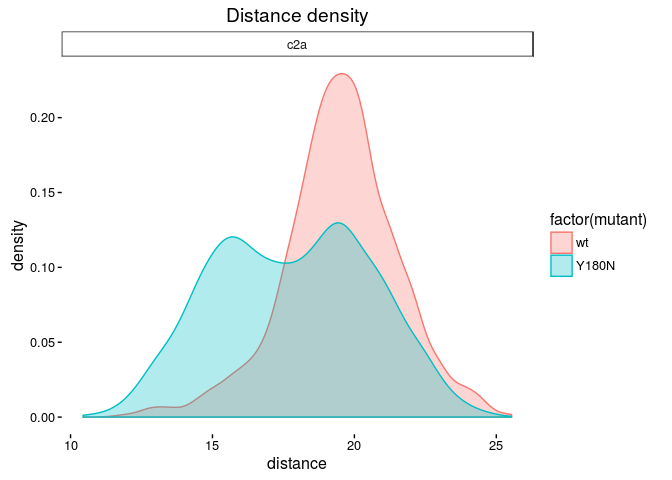
\includegraphics[scale=0.8]{fig.png}
\centering
\end{figure}

\paragraph{Future Objectives}
Continuing on from this summer, I hope to polish and complete the work I've done for publication. 
I plan to extend my work on synaptotagim to dysferlin, a homologous protein, with the intent of elucidating the mechanism
in which C2 mutations lead to dysferlinopathies in humans. Limb-girdle muscular dystrophy is an example
of a dysferlinopathy that we have studied in medical school. I have the opportunity to investigate the
etiology and pathogenesis of this condition using the techniques that I have learned this summer.

\end{document}
